
\begin{frame}{The basic problem}

%\adjincludegraphics[width=0.9\textwidth,trim={0 {.5\height} 0 0 }, clip]{static_figures/survey_and_voting.jpg}

We have a survey population, for whom we observe:
%
\begin{itemize}
 \item Covariates $\x$ (e.g.~race, gender, zip code, age, education level)
 \item Responses $\y$ (e.g.~A binary response to ``do you support Trump'')
\end{itemize}
%

We want the average response in a target population,
in which we observe only covariates.


\splitpage{
    \centering
    \only<1>{
    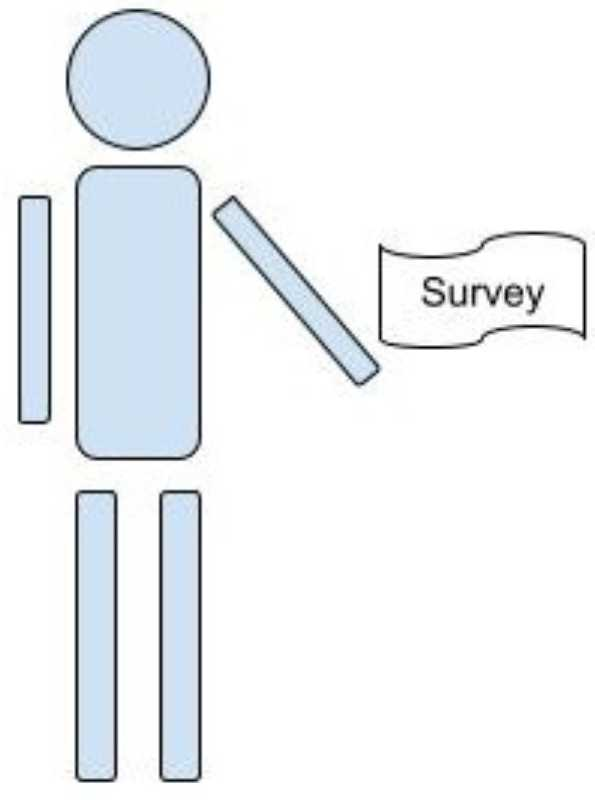
\includegraphics[width=0.5\textwidth]{static_figures/survey_man.jpg}
    }
    \only<2->{
    %
\includegraphics[width=0.5\textwidth]{static_figures/survey_crazy_man.jpg}
    
\includegraphics[width=0.5\textwidth]{static_figures/guinea_pig.png}
    }
}{
    \centering
    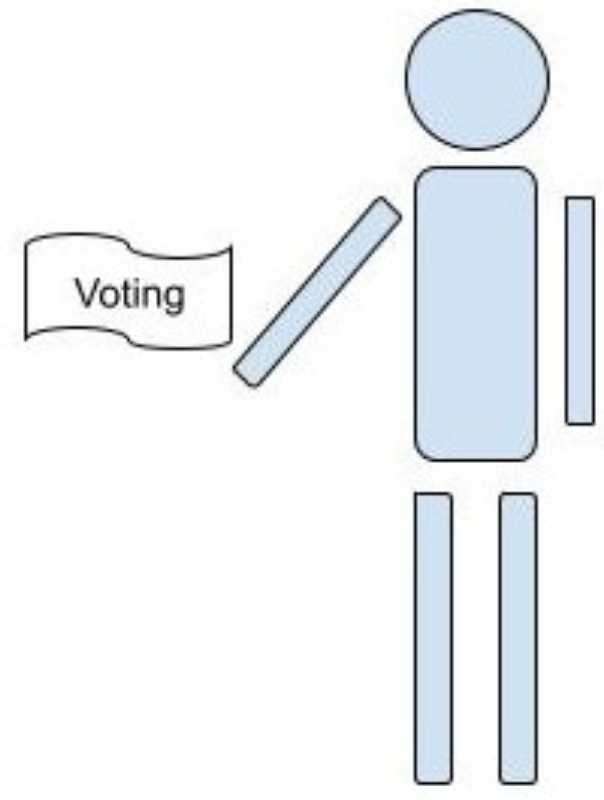
\includegraphics[width=0.5\textwidth]{static_figures/voting_man.jpg}
}

\splitpage{
    \centering
    Observe \surcol{$(\x_i, y_i)$ for $i = 1, \ldots, \nsur$}\\
}{
    \centering
    Observe \tarcol{$\x_j$ for $j = 1, \ldots, \ntar$}\\
}

\onslide<2->{
\textbf{The problem is that the populations may be very different, maybe leading to bias.}
\footnote{Photo copyright: Mark Taylor / \texttt{naturepl.com}}
}

\onslide<3->{
    How can we use the covariates
    to say something about the target responses?
}
%
\end{frame}

%%%%%%%%%%%%%%%%%%%%%%%%%%%%%%%%%%%%%%%%%%%%%%%%%%%%%%%
%%%%%%%%%%%%%%%%%%%%%%%%%%%%%%%%%%%%%%%%%%%%%%%%%%%%%%%
%%%%%%%%%%%%%%%%%%%%%%%%%%%%%%%%%%%%%%%%%%%%%%%%%%%%%%%

\begin{frame}[t]{Two approaches}

We want $\tarcol{\mu := \meantar \y_j}$,
but don't observe target $\tarcol{\y_j}$.  Let $\surcol{\Ysur = \{\y_1, \ldots, \y_{\Nsur}\}}$.

\begin{itemize}
    \item Assume $p(y | \x)$ is the same in both populations,
    \item But the distribution of $\x$ may be different in the survey and target.
\end{itemize}
%
\pause

\splitpagenoline{
    \centering
    \textbf{Calibration weighting (CW)}
}{
    \centering
    %\textbf{Multilevel regression and poststratification (MrP)}
    \textbf{Bayesian hierarchical modeling (MrP)}
}
%
%\\\hrulefill\\
\\[1em]
%
\splitpagenoline{
    \centering
    $\blacktriangleright$
    Choose ``calibration weights'' \surcol{$w_i$}\\
    using only the regressors $\x$\\
    (e.g.~raking weights)
}{
    \centering
    $\blacktriangleright$
    Choose $\expect{}{\y \vert \x, \theta} = m(\theta^\trans \x)$,\\
    choose prior $\p(\theta | \Sigma) \p(\Sigma)$\\
    (e.g.~Hierarchical logistic regression)
} \pause
%
\\[1em]
\splitpagenoline{
    \centering
    $\blacktriangleright$ Take
    $\muhatcw = \surcol{\meansur w_i y_i}$
}{
    \centering
    $\blacktriangleright$ Take
    $\tarcol{\yhat_j} =
        \expect{\postsur}{\y | \tarcol{\x_j}}$ and\\
    $\muhatmrp = \tarcol{\meantar \yhat_j}$
}\pause
%
\\[1em]
\splitpagenoline{
    \centering
    $\blacktriangleright$ Dependence %of \surcol{$\muhat_{\cal}$}
    on \surcol{$\y_i$} is clear\\
    % (\surcol{$\w_i$} typically chosen using only $\x$)
}{
    \centering
    $\blacktriangleright$ Dependence %of \surcol{$\muhat_\mrp$}
    on \surcol{$\y_i$} very complicated\\
    (Typically via MCMC draws from $\postsur$)
}\pause
%
\\[1em]
\splitpagenoline{
    \centering
    $\blacktriangleright$ Weights give interpretable diagnostics:
    %
    \begin{itemize}
        \item Regressor balance
        \item Frequentist variability
        \item Partial pooling
        \item Extraplolation
    \end{itemize}
    %
}{
    \centering
    $\blacktriangleright$ \textbf{Black box}\\
    \pause
    \vspace{1em}
    $\leftarrow$ We open this box, providing analogues of all these diagnostics
}


\end{frame}


%%%%%%%%%%%%%%%%%%%%%%%%%%%%%%%%%%%%%%%%%%%%%%%%%%%%%%%
%%%%%%%%%%%%%%%%%%%%%%%%%%%%%%%%%%%%%%%%%%%%%%%%%%%%%%%
%%%%%%%%%%%%%%%%%%%%%%%%%%%%%%%%%%%%%%%%%%%%%%%%%%%%%%%

\begin{frame}{Prior work: Equivalent weights for linear models}

\textcite{gelman:2007:struggles} observes that MrP is a CW estimator when
one uses linear regression to form $\yhat$:
$$
\begin{aligned}
% \yhat_j ={}& \x_j^\trans \thetahat  =
%     \x_j^\trans \left(\sumsur \x_i \x_i^\trans \right)^{-1} \sumsur \x_i \y_i \Rightarrow \\
\muhatmrp ={}& \tarcol{\meantar \yhat_j} =
\tarcol{\meantar }
\underbrace{\tarcol{\x_j^\trans} \surcol{\thetahat}}_{\textrm{Linear in }\surcol{\Ysur}}
% =
% \surcol{\sumsur}
% \underbrace{
% \left(\tarcol{\meantar \x_j^\trans}
%     \surcol{
%         \left(\sum_{i'=1}^{\Nsur} \x_{i'} \x_{i'}^\trans \right)^{-1} \x_i
%     }
% \right)
% }_{\surcol{\w^\mrp_i}}  \surcol{\y_i} \\
\end{aligned}
$$

Most existing literature on comparing CW and MrP focus on such linear models.
\footnote{
    For example,
    \textcite{gelman:2007:struggles,benmichael:2021:multilevel,chattopadhyay:2023:implied}.}

\onslide<2->{
But what if you use a non--linear link function?  Or a hierarchical model?\\
\vspace{2em}
\hrulefill
\begin{displayquote}
``It would also be desirable to use nonlinear methods  ...
but then it would seem difficult to construct
even approximately equivalent weights.  Weighting and fully nonlinear models
would seem to be completely incompatible methods.''
--- \parencite{gelman:2007:strugglesrejoinder}
\end{displayquote}
}
\vspace{1em}

\end{frame}





% %%%%%%%%%%%%%%%%%%%%%%%%%%%%%%%%%%%%%%%%%%%%%%%%%%%%%%%
% %%%%%%%%%%%%%%%%%%%%%%%%%%%%%%%%%%%%%%%%%%%%%%%%%%%%%%%
% %%%%%%%%%%%%%%%%%%%%%%%%%%%%%%%%%%%%%%%%%%%%%%%%%%%%%%%

% \begin{frame}[t]{Equivalent weights for (some) logistic regression MrP}
% %
% \begin{itemize}
%     \item Suppose the model is $\m(\x^\trans \theta) = \mathrm{Logistic}(\x^\trans \theta)$, with MLE $\thetahat$.
%     \item MrP is $\muhatmrp = \tarcol{\meantar \m(\x_j^\trans \thetahat)}$.
% \end{itemize}

% The map from $\surcol{\Ysur} \mapsto \m(\x_j^\trans \thetahat)$ is
% \emph{inherently nonlinear}.

% But \emph{some sample averages}
% of $\m(\x_j^\trans \thetahat)$ can be approximately linear.\pause

% \begin{block}{Example \#1}
% Additionally suppose $\x \in \mathcal{X}$ is discrete and saturated.
%         \textbf{Then MrP is a CW estimator.}
% \end{block}

% \pause
% \def\ybar{\overline{y}}
% \def\Ntarc{\tarcol{N_T^c}}
% \def\Nsurc{\surcol{N_S^c}}
% %
% \begin{itemize}
%     % \item Let $N_S^c$ (or $\Ntar^c$) denote the \# of survey (or target) observations with $\x_n = c$.
%     % \item When $\x_n = c$, $\m(\x_j^\trans \thetahat) = \frac{1}{\Nsur^c} \sumsur \y_i \ind{\x_n = c}$.
%     \item Let \surcol{$\ybar_S^c$} denote the survey average among $\x = c$ for $c \in \mathcal{X}$\pause
%     \item For $\x = c$, the MLE satisfies $m(\thetahat^\trans \x) = \surcol{\ybar_S^c}$\pause
%     \item Let $\Nsurc$ (or $\Ntarc$) denote the \# of survey (or target) observations with $\x_n = c$.\pause
% \end{itemize}
% %
% $$
% \begin{aligned}
% \muhatmrp ={}& \tarcol{\meantar \m(\x_j^\trans \thetahat)}
%             = \frac{1}{\tarcol{\Ntar}} \sum_{c \in \mathcal{X}}
%             \underbrace{\Ntarc \surcol{\ybar_S^c}}_{\textrm{Linear in }\surcol{\Ysur}}
%         = \surcol{\meansur \w_i^\mrp \y_i}
% \\ \textrm{For }
% \surcol{\w_i^\mrp} ={}&
%     \frac{\Ntarc / \tarcol{\Ntar}}{\Nsurc / \surcol{\Nsur}} \textrm{ when }\x_i=c.
% \end{aligned}
% $$

% \end{frame}


%%%%%%%%%%%%%%%%%%%%%%%%%%%%%%%%%%%%%%%%%%%%%%%%%%%%%%%
%%%%%%%%%%%%%%%%%%%%%%%%%%%%%%%%%%%%%%%%%%%%%%%%%%%%%%%
%%%%%%%%%%%%%%%%%%%%%%%%%%%%%%%%%%%%%%%%%%%%%%%%%%%%%%%

\begin{frame}[t]{Approximately equivalent weights for (some) logistic regression MrP}

\def\alphav{\mathbf{\alpha}}
%
\begin{itemize}
    \item Suppose the model is $\m(\x^\trans \theta) = \mathrm{Logistic}(\x^\trans \theta)$, with MLE $\thetahat$.
    \item MrP is $\muhatmrp = \tarcol{\meantar \m(\x_j^\trans \thetahat)}$.
\end{itemize}

\pause
The map from $\surcol{\Ysur} \mapsto \m(\x_j^\trans \thetahat)$ is
\emph{inherently nonlinear}.

But \emph{some sample averages}
of $\m(\x_j^\trans \thetahat)$ can be approximately linear.
\pause
%
\begin{block}{Example}
Suppose
    $\frac{\tarcol{\ptar}(\x)}{\surcol{\psur}(\x)} \approx \alphav^\trans \x$ for some $\alpha$.
    \textbf{Then MrP is a \emph{approximately} a CW estimator.}
\end{block}

\end{frame}
%%%%%%%%%%%%%%%%%%%%%%%%%%%%%%%%%%%%%%%%%%%%%%%%%%%%%%%
%%%%%%%%%%%%%%%%%%%%%%%%%%%%%%%%%%%%%%%%%%%%%%%%%%%%%%%
%%%%%%%%%%%%%%%%%%%%%%%%%%%%%%%%%%%%%%%%%%%%%%%%%%%%%%%

\begin{frame}[t]{Approximately equivalent weights for (some) logistic regression MrP}

\def\alphav{\mathbf{\alpha}}
%
\begin{itemize}
    \item Suppose the model is $\m(\x^\trans \theta) = \mathrm{Logistic}(\x^\trans \theta)$, with MLE $\thetahat$.
    \item MrP is $\muhatmrp = \tarcol{\meantar \m(\x_j^\trans \thetahat)}$.
\end{itemize}

\begin{block}{Example}
Suppose
    $\frac{\tarcol{\ptar}(\x)}{\surcol{\psur}(\x)} \approx \alphav^\trans \x$ for some $\alpha$.
    \textbf{Then MrP is a \emph{approximately} a CW estimator.}
\end{block}
\pause
$$
\begin{aligned}
\muhatmrp ={}& \tarcol{\meantar \m(\x_j^\trans \thetahat)} \pause
\\ \approx{}&
    \int \tarcol{
        \m(\x^\trans \thetahat) \ptar(\x) d\x
    }
    & \textrm{(Law of large numbers)} \pause
\\ ={}&
    \int
    \surcol{
        \frac{\tarcol{\ptar(\x)}}{\psur(\x)} \m(\x^\trans \thetahat) \psur(\x) d\x
    }
    & \textrm{(Multiply by $\psur(\x) / \psur(\x)$)} \pause
\\ \approx{}&
    \int \surcol{
        \left( \alphav^\trans \x\right) \m(\x^\trans \thetahat) \psur(\x) d\x
    }
    & \textrm{(By assumption)} \pause
\\ \approx{}&
    \surcol{
        \alphav^\trans \meansur \x_i \m(\x_i^\trans \thetahat)
    }
    & \textrm{(Law of large numbers)}\pause
\\={}&
    \surcol{
        \alphav^\trans \meansur \x_i \y_i
    }
    & \textrm{(Property of exponential family MLEs)}
\end{aligned}
$$


\end{frame}


%%%%%%%%%%%%%%%%%%%%%%%%%%%%%%%%%%%%%%%%%%%%%%%%%%%%%%%
%%%%%%%%%%%%%%%%%%%%%%%%%%%%%%%%%%%%%%%%%%%%%%%%%%%%%%%
%%%%%%%%%%%%%%%%%%%%%%%%%%%%%%%%%%%%%%%%%%%%%%%%%%%%%%%

\begin{frame}[t]{Nearly equivalent weights for (some) logistic regression MrP}

\def\alphav{\mathbf{\alpha}}
%
\begin{itemize}
    \item Suppose the model is $\m(\x^\trans \theta) = \mathrm{Logistic}(\x^\trans \theta)$, with MLE $\thetahat$.
    \item MrP is $\muhatmrp = \tarcol{\meantar \m(\x_j^\trans \thetahat)}$.
\end{itemize}
%
\begin{block}{Example}
Suppose
    $\frac{\ptar(\x)}{\psur(\x)} \approx \alphav^\trans \x$ for some $\alpha$.
    \textbf{Then MrP is a \emph{approximately} a CW estimator.}
\end{block}

$$
\begin{aligned}
\muhatmrp =
    \tarcol{\meantar \m(\x_j^\trans \thetahat)} ={}
    \surcol{
        \meansur
        \underbrace{\w_i^\mrp}_{\alphav^\trans \x_i} \y_i
    }  + \textrm{Small error}
\end{aligned}
$$
\pause
But what are the weights?
We don't observe $\frac{\ptar(\x)}{\psur(\x)}$, so can't estimate $\alpha$
directly.\pause

\begin{block}{Key idea (informal)}
\centering
If $\muhatmrp$ is approximately linear, then
$\surcol{\w_i^\mrp} \approx \frac{\partial \muhatmrp}{\partial \surcol{\y_i}}.$\\
\end{block}\pause

For logistic regression, compute and analyze $\frac{\partial \muhatmrp}{\partial \surcol{\y_i}}$
using the implicit function theorem.\footcite{krantz:2012:implicit,giordano:2019:swiss}

\end{frame}



%%%%%%%%%%%%%%%%%%%%%%%%%%%%%%%%%%%%%%%%%%%%%%%%%%%%%%%
%%%%%%%%%%%%%%%%%%%%%%%%%%%%%%%%%%%%%%%%%%%%%%%%%%%%%%%
%%%%%%%%%%%%%%%%%%%%%%%%%%%%%%%%%%%%%%%%%%%%%%%%%%%%%%%

\begin{frame}[t]{Locally equivalent weights for hierarchical logistic regression MrP}
%
\vspace{-1em}
\begin{itemize}
    \item Suppose the model is $\m(\x^\trans \theta) = \mathrm{Logistic}(\x^\trans \theta)$.
    \item Set a hierarchical prior $\p(\theta \vert \Sigma)\p(\Sigma)$,
            use MCMC to draw from $\post$.
    \item MrP is $\muhatmrp = \tarcol{\meantar \expect{\post}{\m(\x_j^\trans \theta)}}$.
\end{itemize}
%
No reason to think $\Ysur \mapsto \muhatmrp$ is even approximately \textbf{globally} linear.

\onslide<2->{
But we can still compute and analyze
$\surcol{\w_i^\mrp} := \frac{\partial \muhatmrp}{\partial \surcol{\y_i}}$
using Bayesian sensitivity analysis!
\footcite{diaconis:1986:bayesconsistency,gustafson:1996:localposterior,efron:2015:frequentist,giordano:2018:covariances}

\begin{block}{MrP weights for MCMC}
\centering
\vspace{-1em}
$$
\begin{aligned}
\surcol{\w_i^\mrp} :={} \frac{\partial \muhatmrp}{\partial \surcol{\y_i}}
=
\tarcol{\meantar}
\underbrace{
    \surcol{
    \cov{\post}{\tarcol{\m(\x_j^\trans \theta)}, \theta^\trans \surcol{\x_i}}
    }
}_{\color{black}\textrm{Can estimate without rerunning MCMC!}}
\end{aligned}
$$
\vspace{-1em}
\end{block}
}

\onslide<3->{
\textbf{What do these weights mean?}  There are now two distinct possibilities:
%
\begin{itemize}
    \item ``Locally implicit weights''
    %
\begin{itemize}
\item An estimator of $\ptar(\x) / \psur(\x)$ (via Riesz regression applied to the Gateaux derivative)
\end{itemize}
%
    \item ``Locally equivalent weights'' \onslide<4->{ $\leftarrow$ \textbf{The present talk will focus on this interpretation}}
\begin{itemize}
\item A characterization of $\Ysur \mapsto \muhatmrp$ for diagnostics and interpretation
\end{itemize}
\end{itemize}
%
}


\end{frame}




%%%%%%%%%%%%%%%%%%%%%%%%%%%%%%%%%%%%%%%%%%%%%%%%%%%%%%%
%%%%%%%%%%%%%%%%%%%%%%%%%%%%%%%%%%%%%%%%%%%%%%%%%%%%%%%
%%%%%%%%%%%%%%%%%%%%%%%%%%%%%%%%%%%%%%%%%%%%%%%%%%%%%%%

\begin{frame}[t]{Locally equivalent weights for hierarchical logistic regression MrP}
%
\vspace{-1em}
\begin{itemize}
    \item Suppose the model is $\m(\x^\trans \theta) = \mathrm{Logistic}(\x^\trans \theta)$.
    \item Set a hierarchical prior $\p(\theta \vert \Sigma)\p(\Sigma)$,
            use MCMC to draw from $\post$.
    \item MrP is $\muhatmrp = \tarcol{\meantar \expect{\post}{\m(\x_j^\trans \theta)}}$.
\end{itemize}
%
\vspace{4em}
%No reason to think $\Ysur \mapsto \muhatmrp$ is even approximately \textbf{globally} linear.
% \onslide<2->{
    \begin{block}{MrP locally equivalent weights (MrPlew)}
    \centering
    \vspace{1em}
    For new data $\Ytil$, form a \textbf{MrP locally equivalent weighting}:
    $$
    \begin{aligned}
    \muhatmrp[\Ytil] \approx{}& \muhatmrp + \surcol{\sumsur \w_i^\mrp (\ytil_i - \y_i)}\quad
    \textrm{where}\quad \surcol{\w_i^\mrp} :={} \frac{\partial \muhatmrp}{\partial \surcol{\y_i}}.
    \end{aligned}
    $$
    \vspace{1em}
    \end{block}
    %
% }

% \only<3>{
%     The weights are given by weighted averages of posterior covariances  \footcite{giordano:2018:covariances}.
%     \\[1em]
%     They can be easily computed with standard software\footnote{We use \texttt{brms} \parencite{brms}.}
%     \textbf{without re--running MCMC}.\\
% }

\vspace{2em}
% \only<4>{
    \textbf{
        Our task is to rigorously show that even such local weights can be meaningfully
        used diagnostically in the same ways we use global weights.
     }
% }



\end{frame}



%%%%%%%%%%%%%%%%%%%%%%%%%%%%%%%%%%%%%%%%%%%%%%%%%%%%%%%
%%%%%%%%%%%%%%%%%%%%%%%%%%%%%%%%%%%%%%%%%%%%%%%%%%%%%%%
%%%%%%%%%%%%%%%%%%%%%%%%%%%%%%%%%%%%%%%%%%%%%%%%%%%%%%%

\begin{frame}{The weights can look very different!}

    \centering
    Does this mean anything?  Are the differences important?

    \AlexanderWeightPlot{}
\end{frame}


